% !TEX TS-program = pdflatex

\documentclass[unicode,11pt,notheorems,xcolor=table]{beamer}
\usepackage{fix-cm}
\usepackage[T2A]{fontenc}
\usepackage[utf8]{inputenc}
\usepackage[russian]{babel}
\usepackage{amsmath,amsfonts,amssymb,amsthm}
\usepackage{mathtools}
\usepackage{diagbox}

\usepackage{ulem}
\usepackage{tikz}
\usepackage{graphicx}
%\usepackage{tkz-graph}
\usetikzlibrary{matrix,arrows,decorations.pathmorphing, arrows.meta,positioning}
\usetikzlibrary{positioning,calc}
\usetikzlibrary{patterns}
\usetikzlibrary{decorations.pathreplacing}

%Описание стиля презентации
\usetheme[sidebar=0]{kfmn} 
\setbeamercovered{transparent}

%\definecolor{cyan}{RGB}{240,217,1}
%\definecolor{vgugreen}{RGB}{143,188,103}
%\definecolor{vgured}{RGB}{234,38,40}
%\definecolor{vgublue}{RGB}{53,101,167}
\hypersetup{colorlinks,linkcolor=,urlcolor=blue}

\makeatletter
	\g@addto@macro{\endtabular}{\rowfont{}}% Clear row font
	\makeatother
	\newcommand{\rowfonttype}{}% Current row font
	\newcommand{\rowfont}[1]{% Set current row font
		\gdef\rowfonttype{#1}#1\ignorespaces%
	}
\makeatother

\newcommand{\myunit}{9mm}
\tikzset{
    node style sp/.style={draw,circle,minimum size=\myunit},
    node style ge/.style={circle,minimum size=\myunit},
    arrow style mul/.style={draw,sloped,midway,fill=white},
    arrow style plus/.style={midway,sloped,fill=white},
}

%[0, 6, 8, 8, 10, 5, 6, 10, 8, 10, 10], 

\pgfdeclareimage[height=8mm]{university-logo}{logo-iem.png}
\logo{\pgfuseimage{university-logo}}
%2[0, 11, 10, 8, 11, 5, 11, 11, 8, 11, 10, 11],

\titlepicture{
	\begin{tikzpicture}[y=1.4cm,overlay,rotate=8]
	\coordinate (O) at (-3cm,0.9cm);
	\filldraw[thick,draw= vgublue, fill=vgublue!20!white] (0,0) circle[radius=4.2cm];
	\clip (0,0) circle[radius=4.2cm];
	\draw (-1.5,1.5) node{
	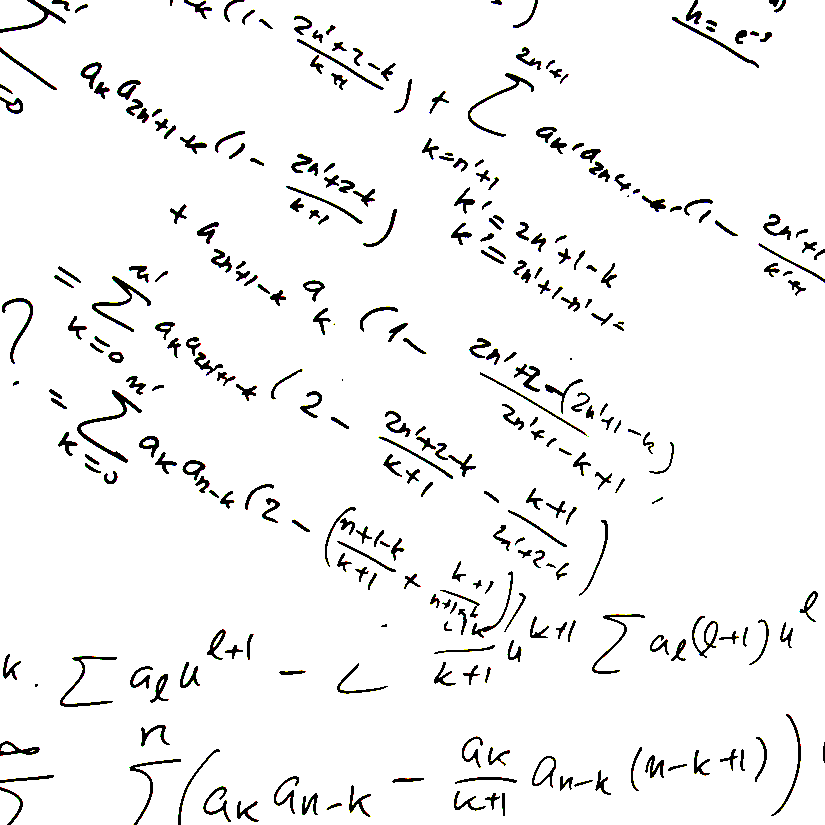
\includegraphics[width=8cm]{titlepic.png}
	};
\end{tikzpicture}
}

\usepackage[math]{iwona}

\newcommand{\hplus}{\mathbin{\hat+}}
\newcommand{\hdot}{\mathbin{\hat\cdot}}
% Описание теорем
\newtheorem{theorem}{Теорема}
\newtheorem{seq}{Следствие}
%%

\LECT % 

% Титульный лист теорем
\author[Д.\,В. Чупраков]{канд.\,физ.-матем.\,наук, доцент Д.\,В. Чупраков\\[6pt] usr10381@vyatsu.ru}

\institute[ВятГУ]{ФГБОУ ВО Вятский государственный университет}

\department{Факультет экономики и финансов}

\title[Лекция~16. Выборочный метод]{
	Введение в экономико-математическое моделирование\\[12pt]
	Лекция~16. Выборочный метод}
\date{9 декабря 2020~г.}


\setbeamercovered{invisible}

\setbeamercolor{math text}{fg=vgured!70!black}


\begin{document}


\maketitle

% \begin{frame}{Структура лекции}{}
% 	\tableofcontents
% \end{frame}

\section{Выборочный метод}

\begin{frame}{Генеральная совокупность}

    Совокупность всех подлежащих изучению объектов или возможных результатов всех мыслимых наблюдений, производимых в неизменных условиях над одним объектом, называется \alert{генеральной совокупностью.}

    \vfill
    \begin{block}{Определение}
        \alert{Генеральная совокупность}~--- это  случайная величина~$X$, заданная на пространстве элементарных событий  с выделенным в нем классом событий, для которых указаны их вероятности.
    \end{block}

    \vfill
    $N$~--- объем генеральной совокупности
\end{frame}

\begin{frame}{Выборка}{}

    \alert{Выборка}~--- совокупность объектов, отобранных случайным образом из генеральной совокупности.
    $n$~--- объем выборки.

    \vfill
    \begin{block}{Определение}
        \alert{Выборка}~--- это последовательность $X_1, X_2,\ldots, X_n$ независимых одинаково распределенных с.в., распределение каждой из которых совпадает с распределением генеральной случайной величины.
    \end{block}

    \vfill
    Метод статистического исследования, состоящий в том, что на основе изучения выборочной совокупности делается заключение о всей генеральной совокупности, называется \alert{выборочным.}

\end{frame}
\begin{frame}{Выборочный метод}{}
    \begin{itemize}
        \item Существенно экономит затраты ресурсов.
        
        \vfill
        \item Дает возможность проведения углубленного исследования за счет расширения программы исследования.

        \vfill
        \item Является единственно возможным в случаях, когда:
        \begin{itemize}
            \item генеральная совокупность бесконечна;
            \item исследование связано с уничтожением наблюдаемых объектов.
        \end{itemize}

        \vfill
        \item Позволяет снизить ошибки регистрации~--- расхождения между истинным и зарегистрированным значениями признака.
    \end{itemize}
\end{frame}
\begin{frame}{Основное свойство выборки}{}
    


    \alert{Репрезентативность}~--- свойство выборки достаточно полно представлять изучаемые признаки генеральной совокупности. 
    
    \vfill
    \begin{block}{Условие обеспечения репрезентативности}
         Все объекты генеральной совокупности должны иметь равные вероятности попасть в выборку.
    \end{block}
\end{frame}


\begin{frame}{Типы выборки}{}

    \begin{itemize}
        \item \alert{Повторная выборка}~--- отобранный объект возвращается в генеральную совокупность перед извлечением следующего;
        \item \alert{Бесповторная выборка}~---  объект не возвращается. 
        
    \end{itemize}        

    \bigskip
    Если объем выборки значительно меньше объема генеральной совокупности, то различие между повторной и бесповторной выборками очень мало.

    \bigskip

    \alert{На практике чаще используется бесповторная выборка.}
\end{frame}

\begin{frame}{Способы отбора}{}
    \begin{itemize}
        \item \alert{простой}~--- из генеральной совокупности извлекают последовательно по одному объекту; 
        \item \alert{типический}~--- генеральную совокупность делят на ,,типы`` и отбор осуществляется из каждой части 
        \item \alert{механический}~--- каждый $t$-й объект генеральной совокупности.
        \item \alert{серийный}~--- объекты из генеральной совокупности отбираются ,,сериями``, которые подвергаются сплошному обследованию.
    \end{itemize}
    
    \bigskip
    На практике пользуются сочетанием вышеупомянутых способов отбора.
\end{frame}

\section{Систематизация наблюдений}


\begin{frame}{Обработка наблюдений}{}
    \begin{block}{Алгоритм}
        \begin{enumerate}
            \item \structure{Формирование выборки:} $X_1,X_2,\ldots, X_n$.
        \item \structure{Исследование выборки:} Получение значений признака
        $$
            X_1=x_1,\quad X_2=x_2,\quad\ldots,\quad X_n=x_n
        $$
    
        Получается набор $(x_1,x_2,\ldots,x_n)$~--- \alert{реализация выборки}.
        $x_i$~--- значение признака.
    
        \item  \structure{Ранжирование вариант}~--- расположениие значений $x_1,\ldots,x_n$ по неубыванию.
    
        \item \structure{Группировка}~---  объединение значений опытных данных в группы так, чтобы в каждой группе признак принимал одно и то же значение.
    \end{enumerate}
\end{block}
     
    \par\medskip\hrule\par \medskip


\end{frame}


\begin{frame}{Связанные понятия}{}
    \begin{itemize}
        \item Конкретные значения $x_1,x_2,\ldots, x_k$ элементов выборки выборки, полученные в результате наблюдений (испытаний) называются \alert{вариантами}.
        
        \item \alert{Вариационный ряд}~--- последовательность вариант $x_1,\ldots, x_k$, расположенных в возрастающем порядке
        $$
            x_1 \leqslant x_2 \leqslant \ldots \leqslant x_k.
        $$
        \item \alert{Статистический ряд}~--- упорядоченная последовательность групп вариант с соответствующими частотами или относительными частотами принадлежности значений группе.
    \end{itemize}
\end{frame}

\begin{frame}{Дискретный статистический ряд}{}
    \begin{block}{}
        \alert{Дискретный статистический ряд}~---  упорядоченная последовательность вариант с соответствующими частотами $n_i$ или относительными частотами $\nu_i$.
    \end{block}

    \bigskip
    \structure{Дискретный ряд частот}
        
    $$
        {\color{black}
        \begin{array}{c|cccc}
            x_i & x_1 & x_2 & \cdots & x_k \\
            \hline
            n_i & n_1 & n_2 & \cdots & n_k \\
        \end{array}
        \qquad \text{где}\quad 
        }
         n_1+n_2+\ldots+ n_k=n
    $$
    \structure{Дискретный ряд частостей (относительных частот)}$\displaystyle\nu_i=\frac{n_i}{n}$
        
    $$
        {\color{black}
        \begin{array}{c|cccc}
            x_i & x_1 & x_2 & \cdots & x_k \\
            \hline
            \omega_i & \nu_1 & \nu_2 & \cdots & \nu_k \\
        \end{array}
        \qquad \text{где}\quad 
        }
        \nu_1+\nu_2+\ldots+ \nu_k=1
    $$
\end{frame}

\begin{frame}{Пример}
    \begin{exampleblock}{}
        В результате тестирования группа студентов в тестированию по математике абитуриентов набрала баллы: 
        $$
            10, 8, 5, 6, 9, 7, 10, 9, 6,10.
        $$
        Записать полученную выборку в виде статистического ряда.   
    \end{exampleblock}
    \begin{itemize}
        \item Проранжируем выборку: $5,6,6,7,8,9,9,10,10,10$
        \item Подсчитаем частоту и частость вариант
        $$
        \begin{array}{|c|c|c|c|c|c|c||c|}
            \hline
            x_i & 5 & 6 & 7 & 8 & 9 & 10 & \Sigma\\
            \hline
            n_i & 1 & 2 & 1 & 1 & 2& 3& 10\\
            \hline
            \omega_i & 0.1 & 0.2 & 0.1 & 0.1 & 0.2& 0.3& 1\\
            \hline
        \end{array}
        $$
    \end{itemize}
\end{frame}
\begin{frame}{Изображение статистического ряда}{}
    Дискретный Вариационный ряд изображается  в виде  \alert{полигона} частот (или частостей)


    \alert{Полигоном частот} называют ломаную, отрезки которой соединяют точки с координатами $(x_i,n_i)$, 
    
    \bigskip 
    \alert{Полигоном частостей}~--- ломаную, отрезки которой соединяют точки с координатами  с координатами $(x_i,\omega_i)$


    \bigskip 
    Варианты $x_i$ откладываются на оси абсцисс, а частоты $n_i$ (частости $\omega_i$)~--- на оси ординат.

\end{frame}

\begin{frame}{Пример}{}
    $$
    \begin{array}{|c|c|c|c|c|c|c||c|}
        \hline
        x_i & 5 & 6 & 7 & 8 & 9 & 10 & \Sigma\\
        \hline
        n_i & 1 & 2 & 1 & 1 & 2& 3& 10\\
        \hline
        \omega_i & 0.1 & 0.2 & 0.1 & 0.1 & 0.2& 0.3& 1\\
        \hline
    \end{array}
    $$
    \bigskip 
    \centering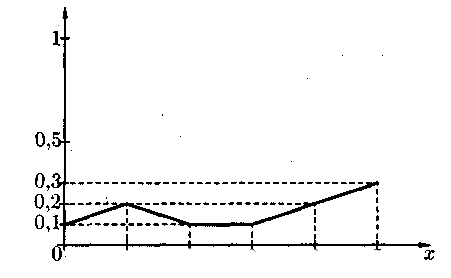
\includegraphics[width=9.5cm]{polygon-1.png}

\end{frame}

\begin{frame}{Статистическое распределение}{}

    \begin{block}{}
    Статистический ряд частостей задает 
    \alert{статистическое распределение}~--- оценку неизвестного распределения~$X$ на~генеральной совокупности. 
    \end{block}
    \vfill
    При больших объемах выборки $n$ статистическое распределение мало отличается от истинного распределения.

    
        % \item  \alert{Интервальный статистический ряд}~--- упорядоченная совокупность интервалов значений случайной величины с соответствующими частотами или относительными частотами попаданий в каждый из них значений величины     
        
        % $$
        % \begin{array}{|c|c|c|c|c||c|}
        %     \hline
        %     x_i & x_1 & x_2 & \cdots & x_k & \Sigma \\
        %     \hline
        %     n_i & n_1 & n_2 & \cdots & n_k & n \\
        %     \hline
        %     \nu_i & \nu_1 & \nu_2 & \cdots & \nu_k & 1 \\
        %     \hline
        % \end{array}
        % $$

    % 
\end{frame}

\begin{frame}{Интервальный статистический ряд}{}
    \begin{block}{}
        \alert{Интервальный статистический ряд}~--- упорядоченная совокупность интервалов значений случайной величины с соответствующими частотами или относительными частотами попаданий значений величины в каждый из них    
    \end{block}
    $$
        {\color{black}
        \begin{array}{c|cccc}
            x_i & \left(x_0,x_1\right] & \left(x_1,x_2\right] & \cdots & \left(x_{k-1},x_k\right] \\
            \hline
            n_i & n_1 & n_2 & \cdots & n_k \\
        \end{array}
        \qquad \text{где}\quad 
        }
         n_1+n_2+\ldots+ n_k=n
    $$

    $$
        {\color{black}
        \begin{array}{c|cccc}
            x_i & \left(x_0,x_1\right] & \left(x_1,x_2\right] & \cdots & \left(x_{k-1},x_k\right] \\
            \hline
            \omega_i & \omega_1 & \omega_2 & \cdots & \omega_k \\
        \end{array}
        \qquad \text{где}\quad 
        }
        \omega_1+\omega_2+\ldots+ \omega_k=1
    $$

\end{frame}


\begin{frame}{Характеристики интервалов}{}
    \begin{itemize}
        \item Число интервалов определяется по формуле Стерджеса
        $$
            k = 1+ [ 3.322\lg{n} ]
        $$

        \item Длина интервала: $h= x_1-x_0 = x_2-x_1=\ldots= x_k-x_{k-1}$ вычисляется как 
        $$
        h= \left[ \frac{x_{\max}-x_{\min}}{3.322\lg{n}} \right]
        $$
        \item Левая граница первого интервала:
        $$
            x_0= x_{\min}-\frac{h}{2}
        $$
    \end{itemize}
\end{frame}

\begin{frame}[t,allowframebreaks]{Пример}{}
    \begin{exampleblock}{}
        Измерили рост (с точностью до см) 30 наудачу отобранных студентов:
        
        153, 154, 155, 155, 156, 157, 158, 159, 160, 163, 164, 165, 166, 167, 167, 169, 170, 171, 171, 172, 173, 173, 175, 175, 178, 179, 179, 182, 183, 186.
       
        Построить интервальный статистический ряд.    
    \end{exampleblock}
    \begin{itemize}
        \item $X$~---рост студента~--- непрерывная с.\,в. 
        \item Данные ранжированы, 
        $$
        n = 30, \qquad x_{\min}=153, \qquad x_{\max}=186
        $$
        \item Вычислим количество интервалов: 
        $$
            k =  1+ [ 3.322\lg 30 ] = 6
        $$
        \vspace{-5mm}
        \item  Находим длину частичного интервала 
        $$
            h = \left[\frac{x_{\max}-x_{\min}}{ 3.322\lg n }\right] = \left[\frac{186-153}{5}\right]= 6
        $$
        
        \vspace{-2mm}
        \item  Находим левую границу:
        $$
         x_0=x_{\min}-\frac{h}{2} = 153-\frac{6}{2} = 150
        $$
        \vspace{-4mm}
        \item Строим интервальный ряд:
    \end{itemize}

    ~\hspace{-8mm}$
    \small
    \begin{array}{|c|c|c|c|c|c|c||c|}
        \hline
        x_i & \left[150; 156 \right) &  \left[156; 162\right) &  \left[ 162; 168 \right) &  \left[ 168; 174 \right) &  \left[174; 180 \right) &  \left[180; 186 \right) & \Sigma\\
        \hline
        x^*_i & 153 &  159 &  165 &  171 &  177 &  183 & \\        
        \hline
        n_i & 4 & 5 & 6 & 7 & 5 & 3 & 30\\
        \hline
        \omega_i & 0,13 & 0,17 & 0,20 & 0,23 & 0,17 & 0,10 & 1\\
        \hline
    \end{array}
    $
\end{frame}



\begin{frame}{Гистограмма}{}
    \begin{block}{Определение}
        \alert{Гистограмма частостей}~--- cтупенчатая фигура, состоящая из прямоугольников, основаниями которых 
        служат частичные интервалы $\left(x_{i-1};x_i\right]$  длиною $h$, а~высоты равны отношению $\frac{\omega_i}{h}$~--- плотности частостей.
    \end{block}
    \begin{minipage}{8cm}
        \centering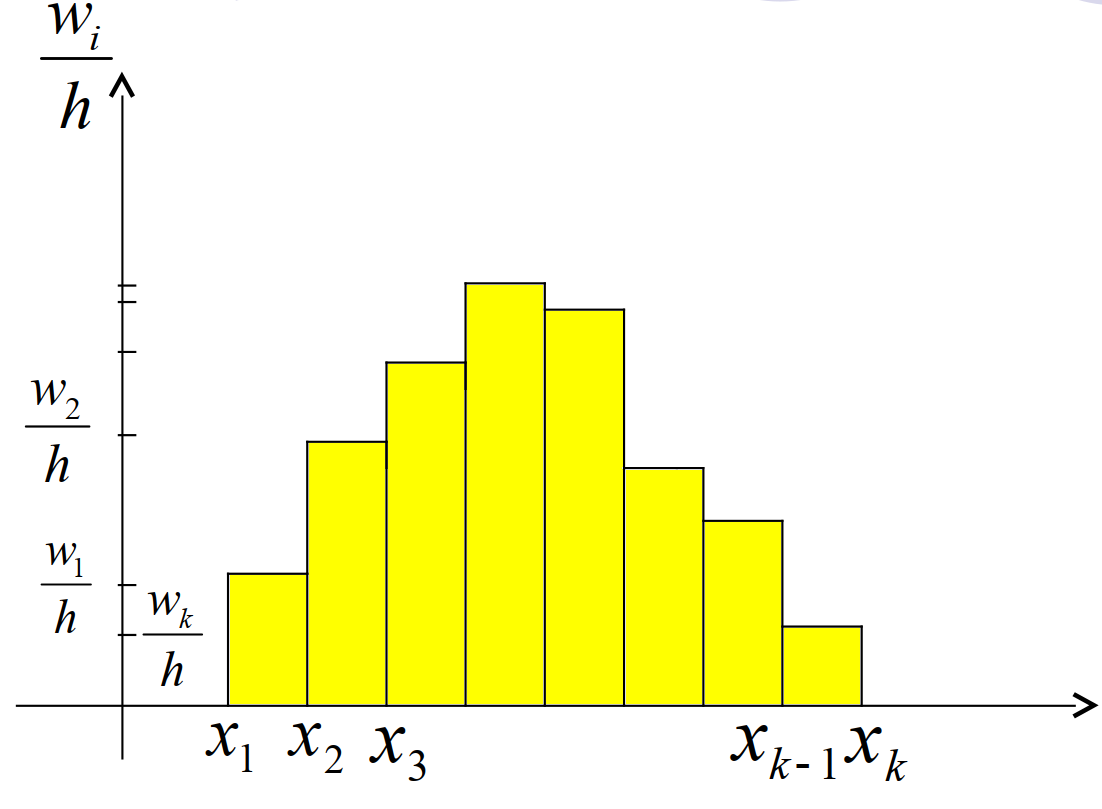
\includegraphics[width=7cm]{hist-1.png}
    \end{minipage}
    \begin{minipage}{2cm}
        {\LARGE
        $$
            S=1
        $$
        \par}
    \end{minipage}
\end{frame}

\begin{frame}{Пример}{}


    ~\hspace{-8mm}$
    \small
    \begin{array}{|c|c|c|c|c|c|c||c|}
        \hline
        x_i & \left[150; 156 \right) &  \left[156; 162\right) &  \left[ 162; 168 \right) &  \left[ 168; 174 \right) &  \left[174; 180 \right) &  \left[180; 186 \right) & \Sigma\\
        \hline
        x^*_i & 153 &  159 &  165 &  171 &  177 &  183 & \\        
        \hline
        n_i & 4 & 5 & 6 & 7 & 5 & 3 & 30\\
        \hline
        \omega_i & 0.13 & 0.17 & 0.20 & 0.23 & 0.17 & 0.10 & 1\\
        \hline
       \dfrac{\omega_i}{h} & 0.022 & 0.033 & 0.038 & 0,23 & 0.028 & 0.017 &\\
        \hline
    \end{array}
    $

    \bigskip 
    \centering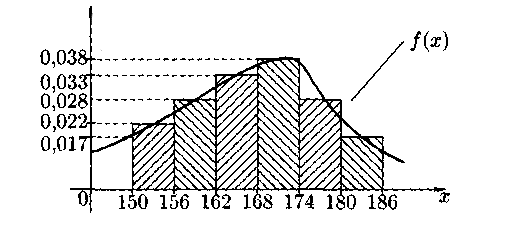
\includegraphics[width=12cm]{hist-2.png}

\end{frame}


\begin{frame}{Числовые характеристики}{}
    
    \begin{itemize}
        \item Средние величины
        \begin{itemize}
            \item Среднее выборочное $\displaystyle \bar{x}_\text{в} = \sum_{i=1}^k \omega_i x_i$
            \item Мода $Mo_\text{в}$~--- значение с наибольшей частотой.
            \item Медиана $Me_\text{в}$~--- значение признака, приходящееся на середину вариационного ряда. 
        \end{itemize}
        
        \vfill
        \item Показатели вариации
        \begin{itemize}
            \item Размах вариации называется число $R=x_{\max}-x_{\min}$
            \item Среднее линейное отклонение: $\displaystyle \bar{x}_\text{в} = \sum_{i=1}^k \omega_i | x_i-\bar{x}_\text{в} |$
            \item Выборочная дисперсия $\displaystyle s^2_\text{в} = \sum_{i=1}^k \omega_i (x_i-\bar{x}_\text{в} )^2$
            \item Среднее квадратическое отклонение 
            $\displaystyle  s_\text{в}= \sqrt{s^2_\text{в}}$
        \end{itemize}
    \end{itemize}
\end{frame}

\begin{frame}{Дополнительне характеристики}{}
    \begin{itemize}
       \item Начальный момент k-порядка:
       $
       \displaystyle \tilde{\nu}_k= \sum_{i=1}^k \omega_i x^k_i
       $
       
       \vfill
       \item Центральный момент $k$-порядка:
       $
       \displaystyle    \tilde{\mu}_k= \sum_{i=1}^k \omega_i (x_i-\bar{x})^k
       $
       
       \vfill\item Коэффициент ассимметрии: 
       $
       \displaystyle   \tilde{A} = \frac{\mu_3}{s^3}
       $

       Если $\tilde{A} = 0$ то распределение симметрично.
        
        \vfill
        \item Эксцесс:            
        $
        \displaystyle  \tilde{\gamma} = \frac{\mu_4}{s^4}-3
        $
        показывает насколько крут вариационный ряд по сравнению с нормальным распределением. 

        Для нормально распределенной величины эксцесс равен 0.
        
        % \vfill
        % \item  Исправленная дисперсия:
        % $$
        % \hat{s}^2_\text{в} = \frac{n}{n-1}s^2_\text{в}
        % $$
        % Используется, чтобы компенсировать смещение дисперсии вследствие применения выборочного метода.
    \end{itemize}
\end{frame}

\begin{frame}{}{}
    Чтобы вычислить характеристики выборочного распределения, заданного интервальным рядом берут представителя каждого интервала~----  значеине, расположенное в его середине.
\end{frame}




\end{document}
